\begin{figure}[h]
\centering
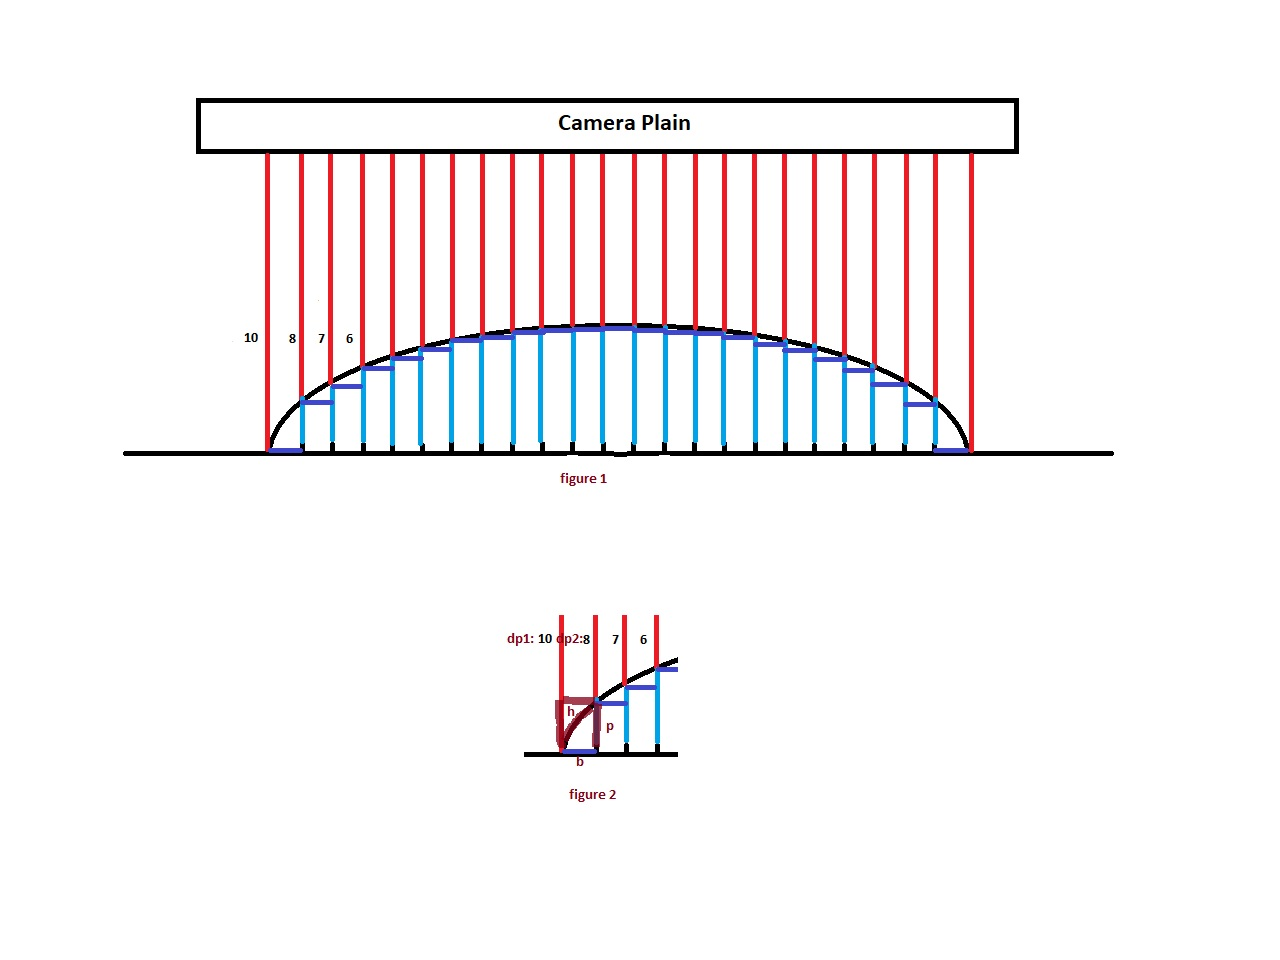
\includegraphics[scale=0.5]{depthToPixels.jpg}
\caption{Heart girth measurement approach}
\end{figure}

Consider figure A.1. Here picture of a surface is taken from a dept camera. Black curve represents the surface and the red lines represent per-pixel distance from camera. Since we assumed that we have a function which can convert number of pixels covered at certain depth to meters, we can get the measures for each pixel in meters. But our problem is to get the length of the length of the curve in meters while preserving the curve, we break the curve into small segments each segment is break after one pixel. If we have to estimate the curve of this segment we can do  so by fitting a triangle on it.  Where base of the triangle is \\ 
\begin{center}
 maxpoint = argmax(depth of P1, depth of P2)  
$b$ = pixelToReal (depth = maxpoint, numberofpixels = 1 ) 
 
\end{center}
Now we have the base in meters we have to calculate the perpendicular or the height this is simply the absolute difference between the depth of P1 and P2 
\begin{center}
 $p$ = \(|depth of P1 -  depth of P2|\) 

\end{center}

once we have the the base and perpendicular we can use the Pythagoras theorem to calculate the hypotenuse or the length of the segment  
\begin{center}

$h=\sqrt{ p^2 + b^2}$ 

\end{center}
						
now we have the formula we can apply this over all segments sum the all segments' length to estimate the length of the curvature. hence by using this technique we can get the the length of heart girth circumference and body length more accurately.
